\documentclass[a4paper]{article}
\usepackage[utf8]{inputenc}
\usepackage{graphicx}
\usepackage{twocolpceurws}
\usepackage{xcolor}
\usepackage{url}

\def\infinity{\rotatebox{90}{8}}

\title{Damegender: Towards an International and Free Dataset about Name, Gender and Frequency}

\author{
David Arroyo Menéndez \\ Grupo de Sistemas y Comunicaciones (GSyC) \\ Universidad Rey Juan Carlos, Madrid, Spain \\ \{d.arroyome@alumnos\}.urjc.es
}

\newif\ifdraft
\drafttrue
%\draftfalse
\newcommand{\nb}[2]{
	{
		{\color{black}{
				\small\fbox{\bfseries\sffamily\scriptsize#1}
				{\sffamily\small$\triangleright~${\it\sffamily\small #2}$~\triangleleft$}
	}}}
}


\ifdraft
\newcommand\davidam[1]{\nb{David}{\color{olive}#1}}
\newcommand\grex[1]{\nb{Gregorio}{\color{red}#1}}
\newcommand\jgb[1]{\nb{Jesús{\color{blue}#1}}}
\newcommand\fixme[1]{{\textcolor{red}{[FIXME] #1}}}
\newcommand\cn{{\color{violet}[citation required]}}

\else
\usepackage[disable]{todonotes}
\newcommand\gema[1]{}
\newcommand\grex[1]{}
\newcommand\mei[1]{}
\newcommand\fixme[1]{}
\newcommand\cn{}


\fi
\let\labelindent\relax
\usepackage[inline]{enumitem}




\institution{URJC}

\begin{document}

\maketitle

\begin{abstract}
  %% Introduction

  Equality of gender is the 5th objective of sustainable development
  in United
  Nations\footnote{https://www.un.org/sustainabledevelopment/gender-equality/}.

  This equality can be reached working on to measure and to analyze
  data and to apply politics from the results. On many gender studies,
  we need to count males and females deciding gender from names, for
  instance, research papers, job positions, streets, ... The
  traditional way is to use commercial APIs with proprietary data
  without idea about how the data has been built. Another way, is
  taking data from Wikipedia, linguistic studies, scientific sites, ...

  %% Methodology

  Many statistical institutions are providing Open Datasets about
  name, gender and frequency. So, we need a scientific discussion
  about unifying formats, making easy ways to process these data and
  ways towards make standards.

  Meanwhile, has been developed Damegender (Free and Open Source
  Software) to retrieve and make calculus with these data.

  %% Results

  The dataset is covering more than 20 countries in the occidental
  world reaching a big number of names and accuracies around (87.56\%)
  with it. Surely, allowing to measure gender gap to students and
  academics interested on the phenomenon without costs and on a
  reproducible way, more people will be contributing to fix the gender
  gap.

  %% Conclusion

  There are a warranty of quality on reproducible research, that's the
  Free Software and the citation about official sources about names,
  gender and frequency provided by statistics institutions making easy
  the peer review and opening doors to the semantic web and the
  attention to diversity.

\end{abstract}

\section{Introduction}
There are a goal in United Nations about gender
gap\footnote{https://www.un.org/sustainabledevelopment/gender-equality/}. What
can I do as software engineer?. The first step is to remember that
``if you cannot measure it, you cannot improve
it"~\cite{thompson1833electrical} and ``Software Engineering Economics
is an invaluable guide to determining software costs, applying the
fundamental concepts of microeconomics to software
engineering~\cite{barry1981software}''. A common profit using Free
Software and Open Data used to be the reduction of costs, for example,
many people and institutions is using LibreOffice and Ubuntu
(GNU/Linux) to avoid the payment by propietary licenses with similar
solutions such as Microsoft Windows and Microsoft Office, the new
costs used to be change a social inertia changing popular products by
products without costs. There are a set of gender detection tools from
the name is based on API solutions, giving a free software and open
data solution, it will be making a competition in a market without a
very strong leader, avoiding payments and thinking on strategies about
profits from a trademark, such as, Firefox or Chrome.

Detecting personal names, you can infer gender on academical papers,
books, newspapers and many interactions on Internet. So, the task
about detect gender from the names could be a strategical task to
measure gender gap.

Nowadays, many people are using APIs such as Genderapi, Genderize,
Namsor, or NameApi. Another people is using solutions based on
Wikipedia, or Free Software solutions (NLTK\cite{loper2002nltk}, R
Gender, Gender Detector, Gender
Computer\footnote{https://github.com/tue-mdse/genderComputer}, ...)

Open Source solutions has a few number of names due to use files of a
single country or being software not maintained in the long time. And
Wikipedia is not taking into account the frequency of the personal
names.

However, the gender gap is a problem recognised in United Nations and
the IT market is leading big inequalities in the world in economy and
gender gap. This paper presents a real work collecting data with a
scientific perspective to solve the problem giving a full toolkit that
is solving a good number of problems (search engine, infer gender in
csv files, names in different countries, wide dataset, ...) faced by
the industry and other problems not solved in an industrial way such
as count males and females in Github repositories, mailing lists, ...

Another previous work~\cite{karimi2016inferring} about this kind of
tools is discussing about the datasets as a way to improve the
accuracies, comparing tools that is using different public datasets
(SSA, IPUMS, namdict, ...)

The solutions is being faced by a practical way: augmenting the number
of names using official statistics and taking into account diversity
goals such as non binary gender and cultural minorities.

With DameGender we will make science
reproducible\cite{peng2011reproducible} in fields where has done
similar works such as Natural Language Processing (gender detection
from the name~\cite{sun2019mitigating}), social sciences or journalism
(gender
gap~\cite{holman2018gender,mislove2011understanding,niemi2017gendered,de2014genero}),
linguistic~\cite{hutson2016gender,van2020gender,okal2018linguistic},
software engineering~\cite{vasilescu2012gender}, ...

The remainder of this paper is structured as follows:

In Section~\ref{sec:stateofart} presents the main research works about
to measure gender gap and gender detection tools from the name.

Section~\ref{sec:design} is giving vocabulary and philosophy about to
choose sources and to face the diversity troubles building a dataset.

Section ~\ref{sec:measuring} explains an application about this
dataset to measure gender gap in GNU/Linux.

Section~\ref{sec:conclusions} points a summary about this approach and
future works.

The contributions to the State of Art presented in this paper are:

1. An integrated solution where make experiments in the different
applications field relative to inferring gender from the name.

2. A collection of Open Datasets retrieved from statistical sources
and standardized in an unique format about gender, name and frequency

3. A new study applying DameGender to count males and females in
GNU/Linux

4. An approach based on reproducible results.


\section{State of Art}
\label{sec:stateofart}

\subsection{About Gender Gap}

Fix the gender gap refers to equality between males and females, it's
about non discrimination policies between males and females. The
gender is about the sex determined in the moment of the birth,
although can be changed in some moment in the life. So, there are
discussions about the gender definition referring to these
problems. But there are consensus determining gender, frequency and
names with official statistics released by the institutions in the
states.

To measure gender gap requires set indicators about it. In
~\cite{world2021global} has been proposed economy, health, education
and politics. And in United Nations\footnote{https://www.unwomen.org/}
there are indicators such as laws, education, mortality of mothers,
political participation, poverty, domestic work, gender parity in
the work, access to economy, situation about the youth (access to
studies and/or work), violence against the women, climate justice,
access to the justice, health, ...

When the measurement has been done with these indicators defined, it's
possible make decisions improving the situation through conclusions
about researches, for example, in ~\cite{miyake2010reducing} are
concluding that making affirmations about ethical values are being
reduced the gender achievement gap in colleges.

Many times, to measure the gender gap has been reached with
methodologies in social research, such as the survey. For example, in
~\cite{bimber2000measuring} has been presented two factors in the
gender gap in Internet (access and use) by socioeconomic and gender
reasons in a survey collecting data for several years. The Internet
access is so important in the economy, education, ... Another work
~\cite{10.1007/978-3-319-39225-7_13} is using a survey of 2000
contributors.

\subsection{Counting Males and Females in Internet. Why? Where?}

This work is focused retrieving data from secondary sources such as
GitHub, Wikipedia, APIs, websites in general, mailing lists, ...
There are serious previous research works about factors modifying
several gender gap indicators (economy, education, politics, ...) from
secondary sources.

For example, a social scientist studying gender gap in
journalism~\cite{alvarez2012journalism} can be counting males and
females in Twitter. These metrics are important because the journalism
is determining gender gap or not in political, education, economy,
... Meanwhile, there are Computer Science making research about how to
count males and females in Twitter~\cite{burger2011discriminating}. On
these works, is being retrieved name, nickname, photo and identifying
gender from these data.

~\cite{burger2011discriminating} has been presenting several
configurations of a language-independent classifier for predicting the
gender of Twitter users. The large dataset used for construction and
evaluation of these classifiers was drawn from Twitter users who also
completed blog profile pages.

And in ~\cite{mislove2011understanding} has been analyzed the Twitter
population including the gender. The gender was inferred making queries
from the names to the dataset provided by US statistic institution.

In ~\cite{wagner2015s} has been analizying the gender gap in Wikipedia
showing evidence of more subtle forms of gender inequality, being
Wikipedia an interesting factor in education, explaining how to solve
these evidences. To measure gender inequality has been developed the
next bias: coverage, structural, lexical (ex: discriminatory words
for women) and visibility.

Computer Science is generating many Forbes billionaires, the public
code is a factor to understand the gender gap about Computer Science
and that's has some importance in economy. The public repositories can
be used to build indicators about economy in Computer Science with
more factors, such as job positions, value of companies, ... In
~\cite{zacchiroli2020gender} has been conducted the first large-scale
longitudinal study of gender imbalance among authors of
collaboratively developed, publicly available code, where
contributions by female authors remain scarce: less that 8 \% of
commits for which we could detect a gender, confirming decades of
gender imbalance in Free/Open Source Software (FOSS). Steffano was
using namdict dataset through of genderguesser to infer gender from
the name. Another work related is ~\cite{vasilescu2015gender}
explaining that women programmers are in the minority in OSS and other
technical teams, although increased gender and tenure diversity are
associated with greater productivity.

In ~\cite{vasilescu2012gender} are exploring the popular Q\&A about
technological stuff called StackOverflow summarizes that the
percentage of women engaged in SO is greatly imbalanced, and men
represent the vast majority of contributors.

And ~\cite{izquierdo2018openstack} are showing data few females
participating contributing code and taking political responsibilities
in OpenStack community.

Related to gender gap in science is so interesting
~\cite{holman2018gender} presenting a code in R where making calls to
genderize api is giving good approaches about how to calculate gender
gap inferring gender from authors name retrieved from arXiv.

\subsection{Automatic approaches to infer gender}

There are several tasks related with infer gender from Internet
sources: hand written, images, documents, names, ...

In ~\cite{liwicki2011automatic} presents a method inferring gender from
hand written texts with a 67.5 \% of accuracy.

Related to infer gender from images~\cite{gallagher2008estimating}
combines image based gender and age classifiers with the cultural
context information provided by first names to recognize people with
no labeled examples with results near to 60 \% of accuracy.

In ~\cite{argamon2003gender} explains that the females uses many more
pronouns and males use many more noun specifiers in a large subset of
the British National Corpus covering a range of genres. So, in
~\cite{koppel2002automatically} is being presented a document
classification system with accuracy of approximately 80 per cent. And
in ~\cite{cheng2011author} exposes a feature selection and a model
built using Machine Learning earning an accuracy of 85.1 per cent
identifying gender from text.

\subsection{Infering gender from the name}

Generally, the tools to infer gender from the name is based on
datasets that is including gender and name as minimum.

In ~\cite{liu2013s} has been presented a method to infer gender from
first names in Twitter, the dataset was built on hand coded by the
agreement of 3 Amazon workers with 50000 Twitter users select at
random out with only 12681 gender labels. The goal of this study was
to determine the incremental value of using the user name as a feature
in gender inference based on tweets.

In ~\cite{mueller2016gender} presents how to infer gender in
Twitter. They are using namdict and us census as datasets. The
features are 'number of consonants', 'number of vowels', 'number of
syllables', 'number of bouba consonants', 'number of bouba vowels',
'number of kiki consonants', 'number of kiki vowels'. The
classification model is using SVM.

\subsection{Other ideas related}

So, in ~\cite{ambekar2009name} was presented a system to classify name
and ethnicity from Open Sources using Machine Learning extracting a
name list from Wikipedia. A more recent work is
~\cite{nadri2021relationship} where is presented NamPrism being
applied to massive software repositories.

Another approach was presented in ~\cite{bollegala2010automatic} a
lexical-pattern-based approach to extract aliases of a given
name. With a set of names and their aliases as training data to
extract lexical patterns. The candidates are ranked using various
ranking scores. And to construct the ranking function was used
ranking Support Vector Machines.

\subsection{Standards related}

ISO/IEC 5218 proposes a norm about coding gender: ``0 as not know'',
``1 as male'', ``2 as female'' and ``9 as not applicable''.

The RFC 6350
(vCard)~\footnote{https://datatracker.ietf.org/doc/html/rfc6350}
where the section Gender has these categories: ``m as male'', ``f as
female'', ``o as other'', ``n as not applicable'' and ``u as
undefined''. Based on this standard the people who is doing web
publishing can use css classes using a web standard such a
h-card~\footnote{https://github.com/microformats/h-card}
microformats. And in the context of to write forms in web interfaces
consider w3
lectures~\footnote{https://www.w3.org/International/questions/qa-personal-names}

\subsection{Summary}

In the State of Art of gender inference is the first name the key
factor to determine gender, although in many contexts there are more
features: surnames, text, images, nicknames, ... The first name can be
useful to infer another stuff such as race, ethnicity or culture, too.

Machine Learning and the previous features selection is being used in
many works, although the discussion about what is the best approach is
an open discussion.

The datasets can be built on hand by human experts, although there are
some Open Datasets used several times in these researches, such as
namdict, or us census.

\section{Design}
\label{sec:design}

\subsection{Truth and Falsehood in names, gender and frequency}
\label{sec:truthandfalsehood}

The current idea in the field is the data about name, gender and
frequency is ok because there are people who is paying by it, or many
people is downloading a product. This intuition is right generally,
although sometimes the people is paying by a bad product due to a good
marketing strategy, a monopoly or there is a fraud, ... Another idea
is the people trust in the government about statistics such as economy,
demography, democracy, ... So the people can trust on names, gender
and frequency. In Damegender, we are trusting in both notions about
truth: the market's point of view and the official statistic's
point of view.

Sometimes there are problems downloading the official statistics, but
there are people who has retrieved these data, for example, with
web scraping. We want classify these files with another idea about
truth.

Another problem arises when the government does little chances in the
data, sometimes communicating it to the users and other times
not. That could be a problem about upgrades, but it's not a problem
with the truth, although it's possible make a trace about these
chances.

With an international free dataset about names, gender and frequency
we can build reproducible science in fields such as Natural Language
Processing (gender detection from the name), social sciences or
journalism (gender
gap~\cite{holman2018gender,mislove2011understanding,niemi2017gendered,de2014genero}),
linguistic~\cite{lawson2005russian,krueger1962mongolian,van2020gender,agyekum2006sociolinguistic,fraser1987lexicon},
software engineering~\cite{vasilescu2012gender}, ...

\subsection{Gender, Language, Nation and Diversity}
\label{sec:diversity}

There are rules and exceptions in the languages to predict if a name
is about male or female when you don't know the name. For example, in
Spanish or English there are more names ending with 'a' classified as
females than classified as males. And Andrea is female in Spain and
male in Italy. So, it's useful to understand the language and culture
associated with a name. Language is close to nation, but there are
differences, for example, in Spain there are several languages basque,
catalan, castillian, ... or the Spanish is the main language in Spain
and in other countries such as Argentina, Mexico, Ecuador, Bolivia,
... So, it would be useful to detect the language and nation from
names and surnames to help to detect gender.

Some countries, such as Spain, are providing free datasets about
surnames but we need more efforts from many countries on this
objective. On other hand, there are previous works to relate name and
surnames with ethnicity using Wikipedia and Machine
Learning~\cite{ambekar2009name}.

\subsection{Damegender Open Datasets Collection}
\label{sec:damegender}

In Damegender, we have unified the different formats to name, gender
and frequency from official sources in these countries: Argentina,
Austria, Australia, Belgium, Canada, Denmark, Germany, Spain, Finland,
France, Great Britain, Ireland, Mexico, New Zealand, Norway, Russia,
Portugal, Slovenia and United States of America.

We have found 2 main criteria counting males and females: number of
births in a year and people using the name in a year. So, we have
divided the files being to able of make merging. The criteria making
the count is: the average of the last twenty years where the data has
been provided. Both criteria are good indicators to understand how
many people is using a name as male or as female.

Later, we have merged these datasets building a free and international
dataset.

We have found open datasets about countries such as Turkey and China
retrieved by other open source developers that is being included in
Damegender, but not in the international dataset. In Turkey the data
has been retrieved using web scraping. And in China the data has been
built by a company in collaboration with the China government and
contributed to R language program. We want compare precision about
this dataset with the commercial solutions to understand the truth
about these datasets.

We have found surnames given by statistical institutions in Spain,
Russia, United States of America and Argentina. So few statistical
institutions is giving surnames. Understanding the diversity problem
with this fact, we have retrieved surnames for all countries from
Wikidata, these datasets contains few surnames being compared with
datasets provided by statistical institutions. Although in names the
diversity problem would be a minor problem we are giving names
retrieved with Wikidata to the public. We are releasing a free dataset
about surnames and frequencies, too.

When the work is finished, we could to rebuild machine learning models
to predict new names and nicknames in any language and culture. The
results is the longest list of public names.

\begin{table}[t]
\footnotesize
\begin{tabular}[]{lcccc}
  \hline
  Dataset & SSA & namdict & NLTK & Damegender \tabularnewline
  males & 91.320 & 48.821 & 2.943 & 278.928 \tabularnewline
  females & 91.320 & 48.821 & 5.001 & 299.870 \tabularnewline
  \hline
\end{tabular}
\caption{Comparison about the number of names between Open Data solutions}
\label{table:DifferentNamesMeasures}
\end{table}

A possible criticism about our idea is the Leslie
Problem\cite{blevins2015jane}: the match between gender and name has
been changing in some years. And the answer is about you need
introduce the age of the person to solve it. The most used use case is
the input is the name and the output must be gender, frequency and
percentage. So, we are deciding without age, surname, ... in the most
of use cases. The idea about this dataset is to be designed for the
most used use case. Although, we can take into account other inputs,
such as surname or age to improve the accuracy. There are many Open
Datasets with names and frequencies classified by years. So, this
problem can be fixed with Open Data, too.

\begin{table}[t]
\footnotesize
\begin{tabular}[]{lcccc}
  \hline
  Dataset  & Accuracy & Precision & Recall & F1-Score  \tabularnewline
  Damegender &  0.8756  & 0.9638    & 1.0    & 0.925  \tabularnewline
  \hline
\end{tabular}
\caption{Several precision measures about the Damegender International Dataset}
\label{table:DifferentAccuracyMeasures}
\end{table}

We have made measurements about the international DameGender dataset,
using as base of truth the dataset explained in
\cite{10.7717/peerj-cs.156} reaching accuracy (0.8756), precision
(0.9638), recall (1.0) and f1-score (0.925).

\subsection{Free APIs for Free Datasets?}
\label{sec:freeapis}

Many websites about Open Data is delivering methods to retrieve Open
Data with a structured format and without costs for the user, such as,
Wikipedia with SPARQL, OpenStreetMap with API rest, ...

We are detecting that the Open Datasets about names, gender and
frequency are being modified one time per year as maximum for each
statistical institution.

Damegender contains python scripts designed to create the
different datasets and publish json files that could be used as a Free
API Rest publishing the json files in sites as github pages, gitlab
pages, or similar sites with free uploads.

\begin{verbatim}
  $ cat DAVID_all.json
  [{
      "name": "DAVID",
      "frequency": 4856689,
      "males": "99.73267796229078 %",
      "females": "0.26732203770922947 %"
  }]
\end{verbatim}

So, we could think that could have Free API Rest about names, gender
and frequency reaching reduce costs to fix the gender gap on a
collaborative way similar to Wikipedia, OpenStreetMap or many Free
Software projects.

\section{Measuring Gender Gap. GNU/Linux as Use Case}
\label{sec:measuring}

With a trust open dataset about names, gender and frequency is too
easy to measure gender gap. Doing cheap to measure gender gap more
students and academic people could work in the fifth Objective
Development Sustainable of United Nations: to delete the gender gap.

This section is divided counting males and females in Debian, GNU and
Linux.

We have reached the csv files from different ways to know the names
about the people in these communities.

When this paper was being wrote in the Debian community all members
must be collaborating with a gpg key, so we can count males and females
from the keyring. The keyring was imported with gpg commands and later
was dumped the keyring in a csv file.

In the moment to write this paper
GNU\footnote{https://www.gnu.org/people/} and
Linux\footnote{https://www.kernel.org/doc/html/latest/process/maintainers}
has websites with the people collaborating in these projects. So,
making web scraping scripts we have downloaded the people and processed
the people to csv files

In Damegender, we have developed csv2gender, a software with a csv
file as input and deploy a statistics graph and/or return the result
of males, females and unknowns about the input.

To make easy to reproduce the experiment we are pasting the commands
used with the version 0.3.4 of Damegender.

\begin{verbatim}
python3 csv2gender.py files/gnu.csv
 --first_name_position=0
 --title="GNU maintainers grouped by gender"
 --dataset="inter"
 --outcsv="files/gnu.gender.csv"
 --outimg="files/gnu.gender.png"
 --noshow --delete_duplicated

python3 csv2gender.py files/linux.csv
 --first_name_position=0
 --title="Linux maintaners grouped by gender"
 --dataset="inter"
 --outcsv="files/linux.gender.csv"
 --outimg="files/linux.gender.png"
 --noshow --delete_duplicated

python3 csv2gender.py files/debian.csv
 --first_name_position=0
 --title="Debian maintaners grouped by gender"
 --dataset="inter"
 --outcsv="files/debian.gender.csv"
 --outimg="files/debian.gender.png"
 --noshow --delete_duplicated
\end{verbatim}

\begin{figure}
  \centering
  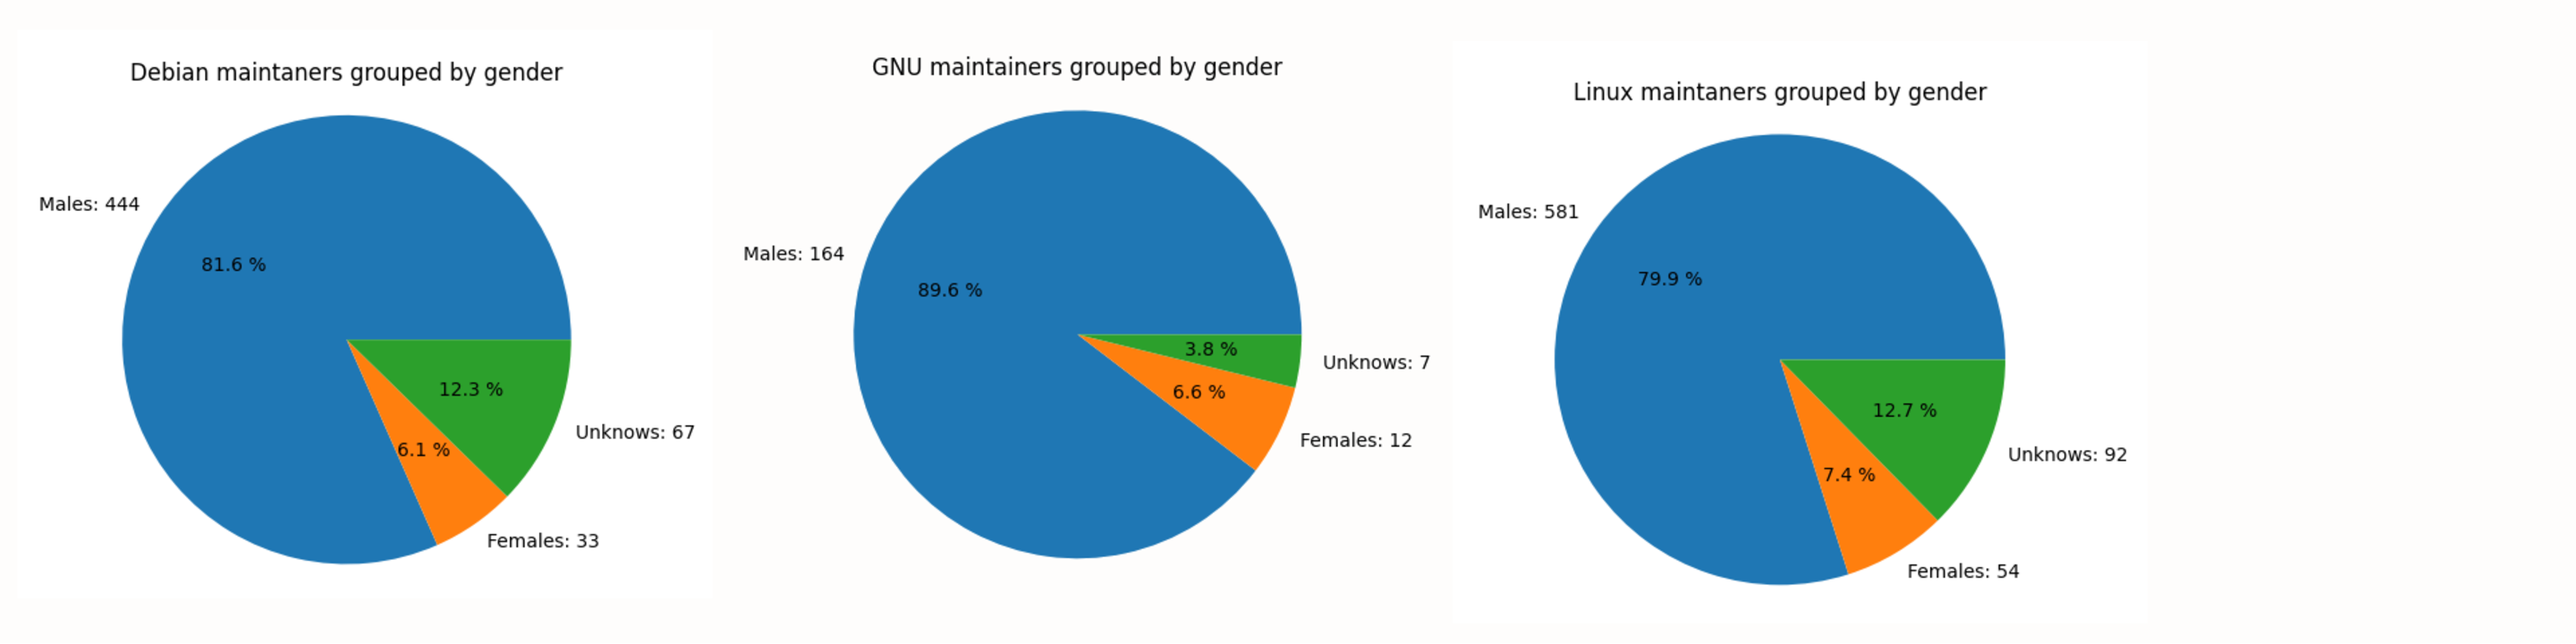
\includegraphics[width=0.6\textwidth]{images/debian-gnu-linux.pdf}
  \caption[Caption for LOF]{Males (blue), Females (orange) and Unknows (green) in Debian, GNU and Linux}
\end{figure}

The inter dataset was created merging several open datasets downloaded
from official statistics sites from different nations: Austria,
Australia, Belgium, Canada, Germany, Denmark, Spain, Finland, Ireland,
Iceland, Mexico, New Zealand, Portugal, Slovenia, United States of
America, Uruguay and France. That's a good representation of the
Western World and the Free Software world is populating this world's
area\cite{gonzalez2008geographic}.

Linux divides the developers in 537 males (73.9\%), 98 females
(13.5\%) and 92 unknowns (12.7\%). The number of unknowns is due to
different reasons, but it's so common in Linux that the developer is a
company and not a name of a person.

GNU divides the developers in 164 males (89.6\%), 12 females (6.6\%)
and 7 unknowns (3.8\%)

The GNU people has a number lowest in females, they are the founder of
the Free Software philosophy, the Debian principles and the Open
Source philosophy was invented later influenced by GNU with very
similar practical decisions (for example: deciding licenses for the
software). Richard Stallman returned to be president recently
apologizing by his personal behaviour with the
females.\footnote{https://www.fsf.org/news/rms-addresses-the-free-software-community}

Debian is a distribution, the project who makes the CD/DVD and the
software ready to be downloaded from Internet with the
dependencies. There are many distributions, such as, Ubuntu or RedHat
so it is not representative, but it's interesting to understand that
the numbers are similar in Debian dividing the developers in 408 males
(75\%), 69 females (12.7\%) and 67 unknowns (12.3\%).

%% \includegraphics[width=0.9\textwidth]{images/debian.gender.pdf}

\section{Conclusions and Future Works}
\label{sec:conclusions}

This paper is explaining the application about Damegender, the
motivations (reproducible research, fix gender gap to reach an
objective of United Nations, fields of application: linguistic, social
sciences, software engineering, natural language processing,
journalism, ...)

A good improvement is to build an international, universal and free
dataset about names, gender and frequency with the right design with
the current state of the job, attending to the diversity (LGBT
options, cultural minorities, ...).

This paper has explained what technologies is involved on reduce costs
about gender gap (gender detection from the names, api rest, semantic
web, ...)

Augmenting the number of countries with statistical institutions
giving names, gender and frequencies with Open Data will be augmenting
the accuracies and giving more attention to the diversity.

The current state of work is the longest Open Dataset about names,
gender and frequency with more than 20 countries representing the
Western World, being a solution with low number of unknowns in the real
world.

The future works is about changes in the big software industry.

Making searches with strings about personal names (ex: Leticia) in
search engines such as Google, these strings are not being classified
as personal names, one solution will be data structured such as
JSON-LD, microdata, microformats, rdfa ... Another solution will be
store in the servers the Open Data Collection about names, gender and
frequency and identify the context about the string is a personal
name, that's an easy problem in popular sites such as Wikipedia,
academic websites, ...

If the search engine identify the string as personal name, it can help
to the user about the gender. That is similar than other problems such
as streets, products, ... where you are giving additional information
such as maps in streets or prices in products.

Other sites such as Github or Gitlab could be giving data about
gender of developers in the site or in the software project with these
datasets.

Another industry is about match sites (Meetic, Tinder, ...) where only
is important photos, age and gender generally. It could be possible to give
to users gender, photo and interests from personal names our open data
collection and information related in Internet.

%% These data reveals that the situation has been improved with respect
%% the long time. In \cite{10.1007/978-3-319-39225-7_13} speaks about a
%% female participation of around 2 {\%} to 5 {\%}.

%% \section*{Acknowledgments}

%% We would like to thank: Statistical institutions by release Open
%% Datasets about names, gender and frequency. Daniel Izquierdo and Laura
%% Arjona for starting this research field at URJC all those working with
%% Jesus González Barahona and Gregorio Robles.

\bibliographystyle{alpha}
\bibliography{uc3m}

\end{document}
